\documentclass[12pt, a4paper]{report}
\usepackage[utf8]{inputenc}
\usepackage[T1]{fontenc}
\usepackage[utf8]{inputenc}
\usepackage{geometry}
\usepackage{listings}
\usepackage{xcolor}
\usepackage[]{graphicx}
\usepackage[export]{adjustbox}
\usepackage{subcaption}


\definecolor{codegreen}{rgb}{0.26, 0.61, 0}
\definecolor{codegray}{rgb}{0.5,0.5,5}
\definecolor{codepurple}{rgb}{58,0,0.82}
\definecolor{backcolour}{rgb}{0.80, 0.81, 0.93}

\lstdefinestyle{mystyle}{
    backgroundcolor=\color{backcolour},   
    commentstyle=\color{codegreen},
    keywordstyle=\color{magenta},
    numberstyle=\tiny\color{codegray},
    stringstyle=\color{codepurple},
    basicstyle=\ttfamily\footnotesize,
    breakatwhitespace=false,         
    breaklines=true,                 
    captionpos=b,                    
    keepspaces=true,                 
    numbers=left,                    
    numbersep=5pt,                  
    showspaces=false,                
    showstringspaces=false,
    showtabs=false,                  
    tabsize=2
}

\lstset{style=mystyle}


\title{\textbf{EE2703: Applied Programming Lab\\Assignment 4\\Fourier Approximations
}}


\author{Devaganthan S S\\ EE19B018}
\date{\today}
\begin{document}

\maketitle


\section{Abstract}
This experiment aims to find the Fourier coefficients of coscos(x) and exp(x) using python by Integration and Least Squares Method and compare the results obtained by plotting them.

\section{Introduction}
We try to reconstruct two functions, $exp(x)$ and $cos(cos(x))$ over the the interval $[0,2\pi)$ using the Fourier series,
\
\begin{equation}\label{eq:4}
a_0 + \ \sum_{n=1}^{\infty} \{a_ncos(nx)+b_nsin(nx)\} \	
\end{equation}
The coefficients $a_k$ and $b_k$ are obtained by integration, using the function{\fontfamily{cmss}\selectfont
'quad().'
}They are also obtained by the least-squares method using the function {\fontfamily{cmss}\selectfont
'lstsq()'
}
\section{Implementation}
The program prints a set of instructions. Based on the requirement, input has to be given. The program can accept multiple Keys, but they have to be separated by ‘,’. For eg. “2,3,7”.

\section{Results}
\subsection{0.1	Plotting the Functions}
The functions $coscos(x)$ and $exp(x)$ are plotted over the interval [0,2$\pi$). Since $exp(x)$ grows rapidly, {\fontfamily{cmss}\selectfont
'semilogy()'
} is used to plot. The function $coscos(x)$ is periodic, whereas the function $exp(x)$ is not. Since we require periodic functions for the Fourier series, for exp(x), we take the interval [0,2$\pi$), and assume it repeats. The below code accomplishes the above.
\
\noindent
\lstinputlisting[language = python]{codeblock1.py}
The plots obtained are,
\begin{figure}[h!]

\begin{subfigure}{0.55\textwidth}
    \centering
    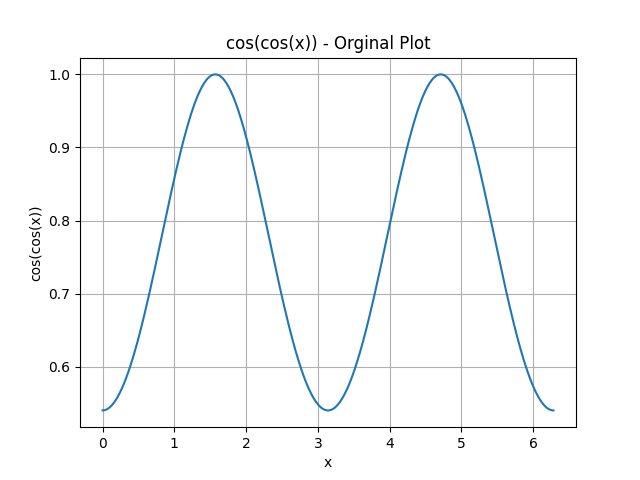
\includegraphics[scale=0.9,width=\linewidth]{figure1.png} 
    \caption{Figure 1}
    \label{fig:my_label}
\end{subfigure}
\begin{subfigure}{0.55\textwidth}
    \centering
    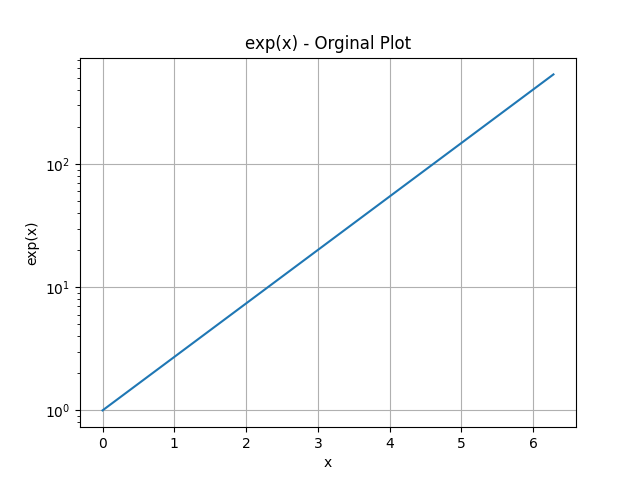
\includegraphics[scale=0.9,width=\linewidth]{figure2.png} 
    \caption{Figure 2}
    \label{fig:image2}
\end{subfigure}


\end{figure}


\subsection{Generating the Coefficients by Integration}
The First 26 ‘a’ coefficients and the  25 ‘b’ coefficients are generated. The below code generates the coefficients for $exp(x)$,
\lstinputlisting[language = python]{codeblock2.py}
For $cos(cos(x))$
\lstinputlisting[language = python]{codeblock3.py}
 

\subsection{Plotting the magnitude of Coeffecients Obtained from Integ}
For the obtained coefficients, the magnitude vs n plot is plotted using {\fontfamily{cmss}\selectfont
'semilogy()'
} and {\fontfamily{cmss}\selectfont
'loglog()'
} functions. The below code accomplishes the above,
\vspace{4mm}
\lstinputlisting[language = python]{codeblock4.py}
The Plots Obtained are,
\vspace{25mm}
\begin{figure}[h!]

\begin{subfigure}{0.55\textwidth}
    \centering
    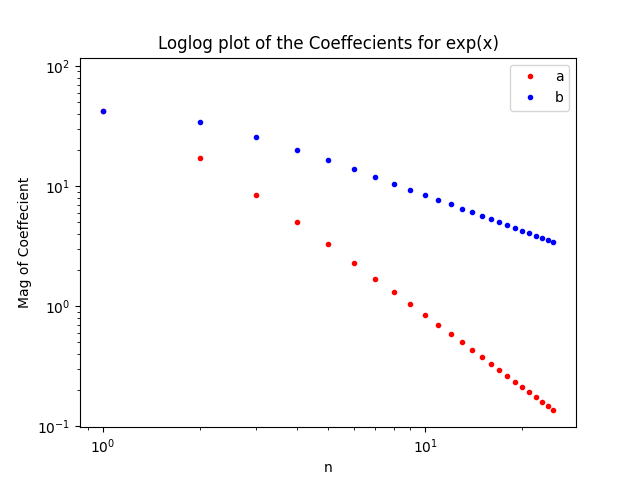
\includegraphics[scale=0.9,width=\linewidth]{fig3.png} 
    \caption{Figure 3}
    \label{fig:my_label}
\end{subfigure}
\begin{subfigure}{0.55\textwidth}
    \centering
    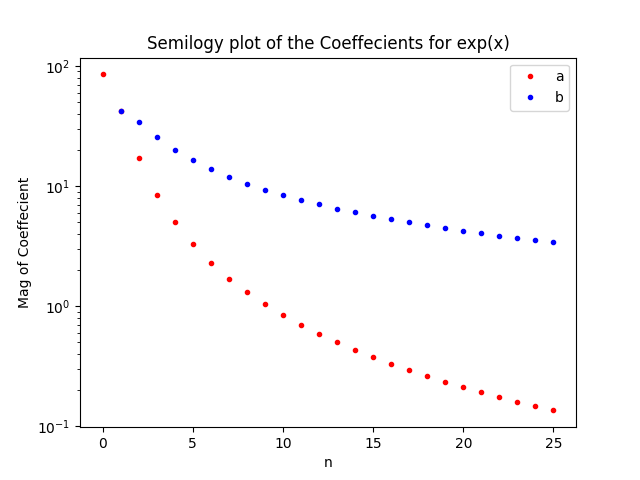
\includegraphics[scale=0.9,width=\linewidth]{fig4.png} 
    \caption{Figure 4}
    \label{fig:image2}
\end{subfigure}


\end{figure}
\begin{figure}[h!]

\begin{subfigure}{0.55\textwidth}
    \centering
    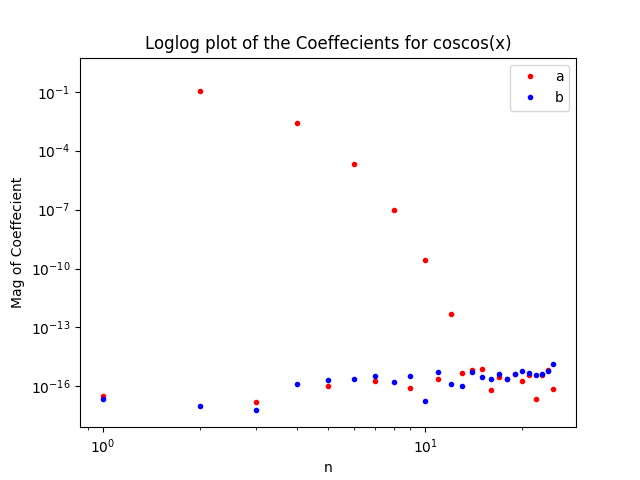
\includegraphics[scale=0.9,width=\linewidth]{fig5.png} 
    \caption{Figure 5}
    \label{fig:my_label}
\end{subfigure}
\begin{subfigure}{0.55\textwidth}
    \centering
    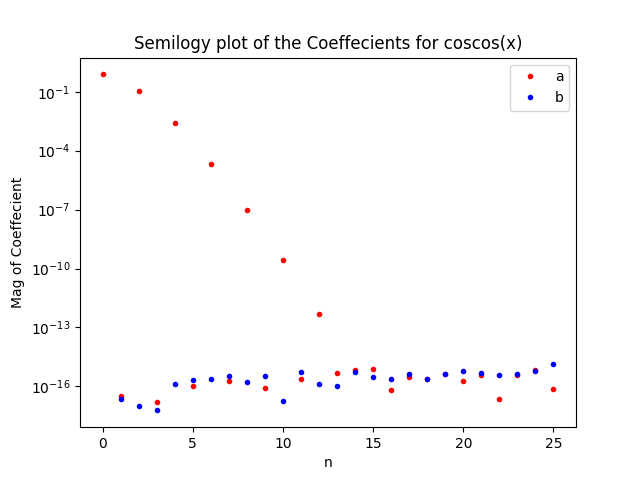
\includegraphics[scale=0.9,width=\linewidth]{fig6.png} 
    \caption{Figure 6}
    \label{fig:image2}
\end{subfigure}
\end{figure}

\
From the fig 5 and fig 6 we can see that $b_n$ coefficients are nearly zero. This happens because $cos(cos(x))$ is an odd function. In the first case, the coefficients do not decay as quickly as the coefficients for the second case because, $exp(x)$ requires infinite number of cos and sin terms, whereas $cos(cos(x))$ does not.
 

\subsection{Plotting the magnitude of Coefficients Obtained from lstsq()}
For the obtained coefficients, the magnitude vs n plot is plotted using {\fontfamily{cmss}\selectfont
'semilogy()'
} and {\fontfamily{cmss}\selectfont
'loglog()'
} functions. The code is similar to as given in section 0.4.3, with only the second argument for the plot functions are the coefficients  obtained from {\fontfamily{cmss}\selectfont
lstsq()
}.The Plots Obtained are,
 \begin{figure}[h!]

\begin{subfigure}{0.55\textwidth}
    \centering
    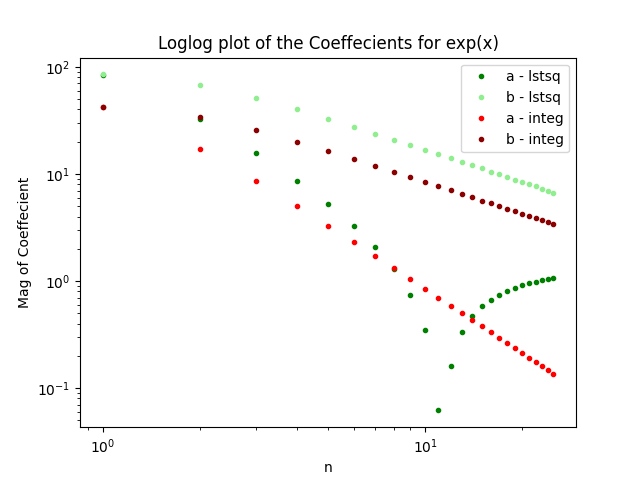
\includegraphics[scale=0.9,width=\linewidth]{fig7.png} 
    \caption{Figure 7}
    \label{fig:my_label}
\end{subfigure}
\begin{subfigure}{0.55\textwidth}
    \centering
    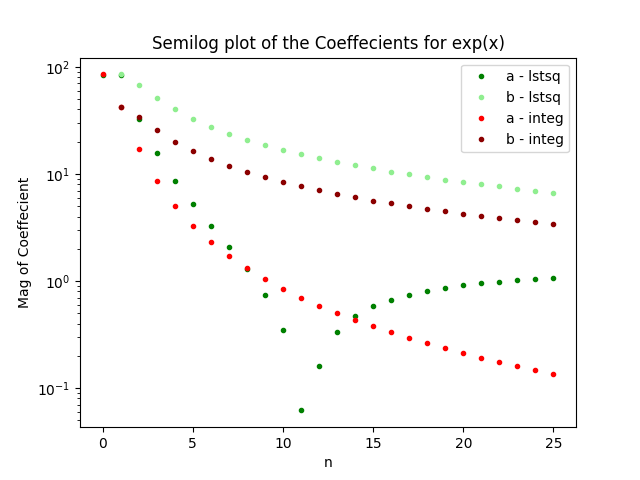
\includegraphics[scale=0.9,width=\linewidth]{fig8.png} 
    \caption{Figure 8}
    \label{fig:image2}
\end{subfigure}


\end{figure}
\begin{figure}[h!]

\begin{subfigure}{0.55\textwidth}
    \centering
    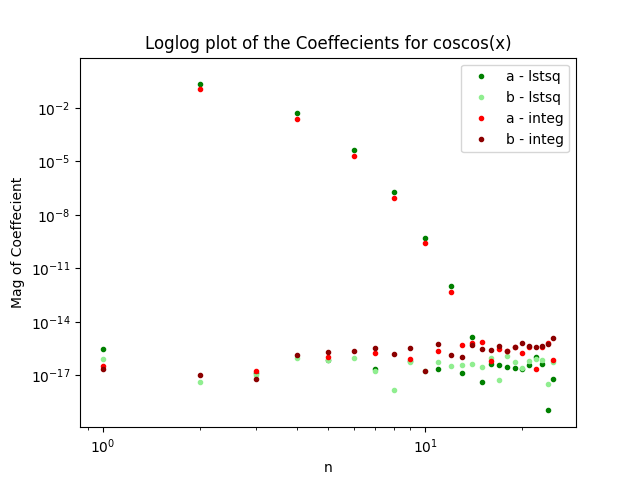
\includegraphics[scale=0.9,width=\linewidth]{fig9.png} 
    \caption{Figure 9}
    \label{fig:my_label}
\end{subfigure}
\begin{subfigure}{0.55\textwidth}
    \centering
    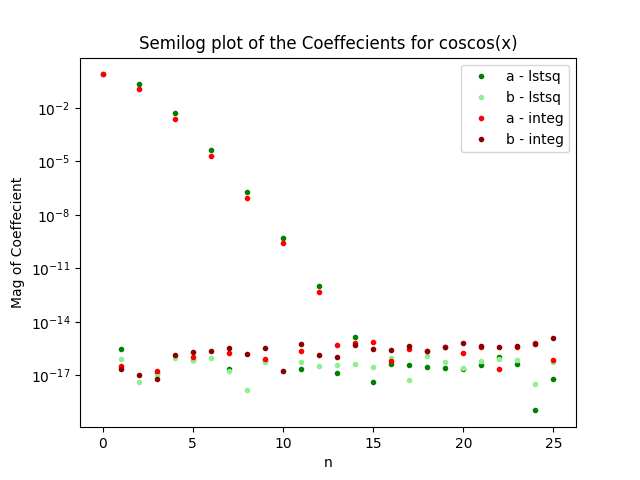
\includegraphics[scale=0.9,width=\linewidth]{fig10.png} 
    \caption{Figure 10}
    \label{fig:image2}
\end{subfigure}
\end{figure}

\
\subsection{Comparing the Coefficients}
The coefficients obtained from the 2 methods do not agree. The least-square method gives 51 coefficients that best approximate the function. Whereas the coefficients obtained from Integration, do not give a best approximate, because they need other coefficients (coefficients other than the 51 computed), to best approximate the function. The below code computes the deviation in each coefficient and also prints the largest deviation. 
\vspace{10mm}
\lstinputlisting[language = python]{codeblock6.py}
\subsection{Reconstructing the Function and Plotting using the Coefficients}
With the Coefficients obtained from both the methods, the function is reconstructed. The reconstructed functions are plotted along with the original function, for the interval, [0,2$\pi$). The below code accomplishes the above for $exp(x)$. For $cos(cos(x))$ the code is the same, with a different set of coefficients.
\
\noindent
\lstinputlisting[language = python]{codeblock7.py}
\vspace{4mm}
The plots obtained are,
\begin{figure}[t]

\begin{subfigure}{0.55\textwidth}
    \centering
    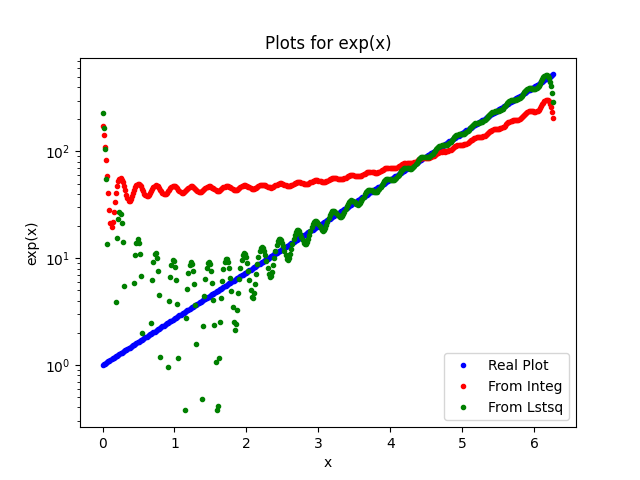
\includegraphics[scale=0.5,width=\linewidth]{fig11.png} 
    \caption{Figure 11}
    \label{fig:my_label}
\end{subfigure}
\begin{subfigure}{0.55\textwidth}
    \centering
    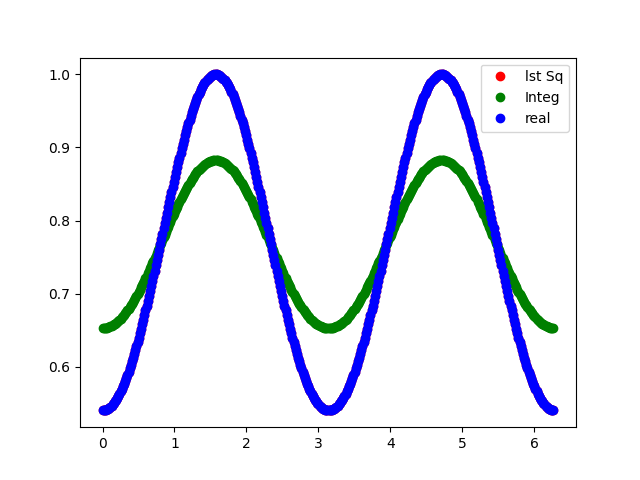
\includegraphics[scale=0.5,width=\linewidth]{fig12.png} 
    \caption{Figure 12}
    \label{fig:image2}
\end{subfigure}
\

The reconstruction of cos(cos(x)) is nearly perfect while exp(x) is not. The reason is that cos(cos(x)) can be written as a sum of a finite number of scaled harmonics while exp(x) cannot.
\end{figure}
\section{Conclusion}
51 Coefficients for both the function are found using the Integration method. The best approximate for the 2 functions, constraining to 51 coefficients are found using the least square method.
\end{document}

